%
% paradox.tex -- template for standalon tikz images
%
% (c) 2019 Prof Dr Andreas Müller, Hochschule Rapperswil
%
\documentclass[tikz]{standalone}
\usepackage{amsmath}
\usepackage{times}
\usepackage{txfonts}
\usepackage{pgfplots}
\usepackage{csvsimple}
\usetikzlibrary{arrows,intersections,math}
\begin{document}
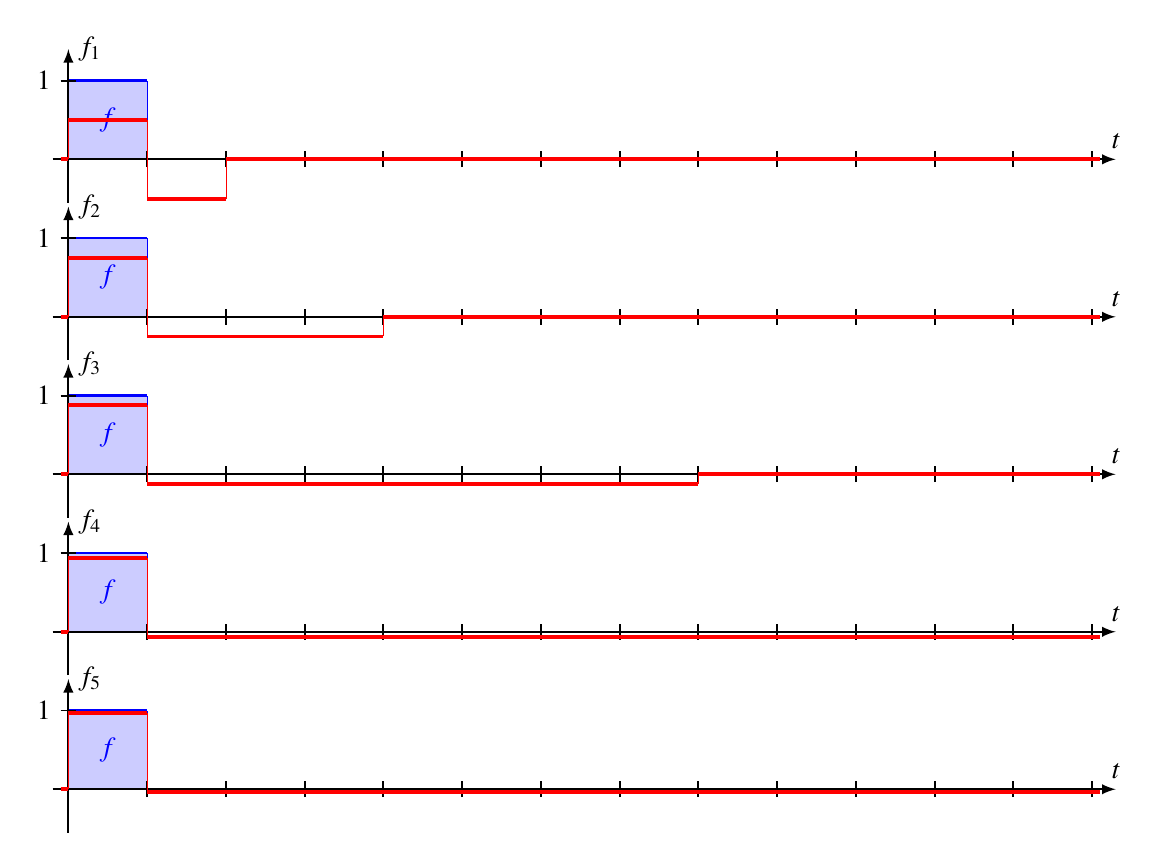
\begin{tikzpicture}[>=latex]

\def\bild#1#2#3{
\fill[color=blue!20] (0,0)--(1,0)--(1,1)--(0,1)--cycle;
\draw[color=blue,line width=1pt] (-0.1,0)--(0,0);
\draw[color=blue,line width=0.1pt] (0,0)--(0,1);
\draw[color=blue,line width=1pt] (0,1)--(1,1);
\draw[color=blue,line width=0.1pt] (1,0)--(1,1);
\node[color=blue] at (0.5,0.5) {$f$};
\draw[->,line width=0.7pt] (-0.2,0)--(13.3,0) coordinate[label={$t$}];
\foreach\x in {1,...,13}{
	\draw[line width=0.7pt] (\x,-0.1)--(\x,0.1);
}
\draw[->,line width=0.7pt] (0,-0.55)--(0,1.4) coordinate[label={right:$f_#3$}];
\draw[line width=0.7pt] (-0.1,1)--(0.1,1);
\node at (-0.1,1) [left] {$1$};
\draw[line width=1.4pt,color=red] (-0.1,0)--(0,0);
\xdef\yold{0}
\xdef\y{#1}
\draw[line width=0.1pt,color=red] (0,\yold)--(0,\y);
\draw[line width=1.4pt,color=red] (0,\y)--(1,\y);
\xdef\yold{\y}
\pgfmathparse{#1-1}
\xdef\y{\pgfmathresult}
\ifnum #2 < 13
	\draw[line width=0.1pt,color=red] (1,\yold)--(1,\y);
	\draw[line width=1.4pt,color=red] (1,\y)--(#2,\y);
	\xdef\yold{\y}
	\xdef\y{0}
	\draw[line width=0.1pt,color=red] (#2,\yold)--(#2,\y);
	\draw[line width=1.4pt,color=red] (#2,\y)--(13.1,\y);
\fi
\ifnum #2 > 13
	\draw[line width=0.1pt,color=red] (1,\yold)--(1,\y);
	\draw[line width=1.4pt,color=red] (1,\y)--(13.1,\y);
\fi
}

\bild{0.5}{2}{1}

\begin{scope}[yshift=-2cm]
\bild{0.75}{4}{2}
\end{scope}

\begin{scope}[yshift=-4cm]
\bild{0.875}{8}{3}
\end{scope}

\begin{scope}[yshift=-6cm]
\bild{0.9375}{16}{4}
\end{scope}

\begin{scope}[yshift=-8cm]
\bild{0.96875}{16}{5}
\end{scope}

\end{tikzpicture}
\end{document}

